
\begin{exercise}

% !TEX root = ../main.tex



\pt{4}\begin{minipage}[t]{.6\linewidth}
	Wat klopt er fysisch niet aan wat er gebeurt in de cartoon? Licht toe.
\end{minipage}
\hfill
\begin{minipage}[t]{.37\linewidth}
	\raisebox{6ex-\height}{%
		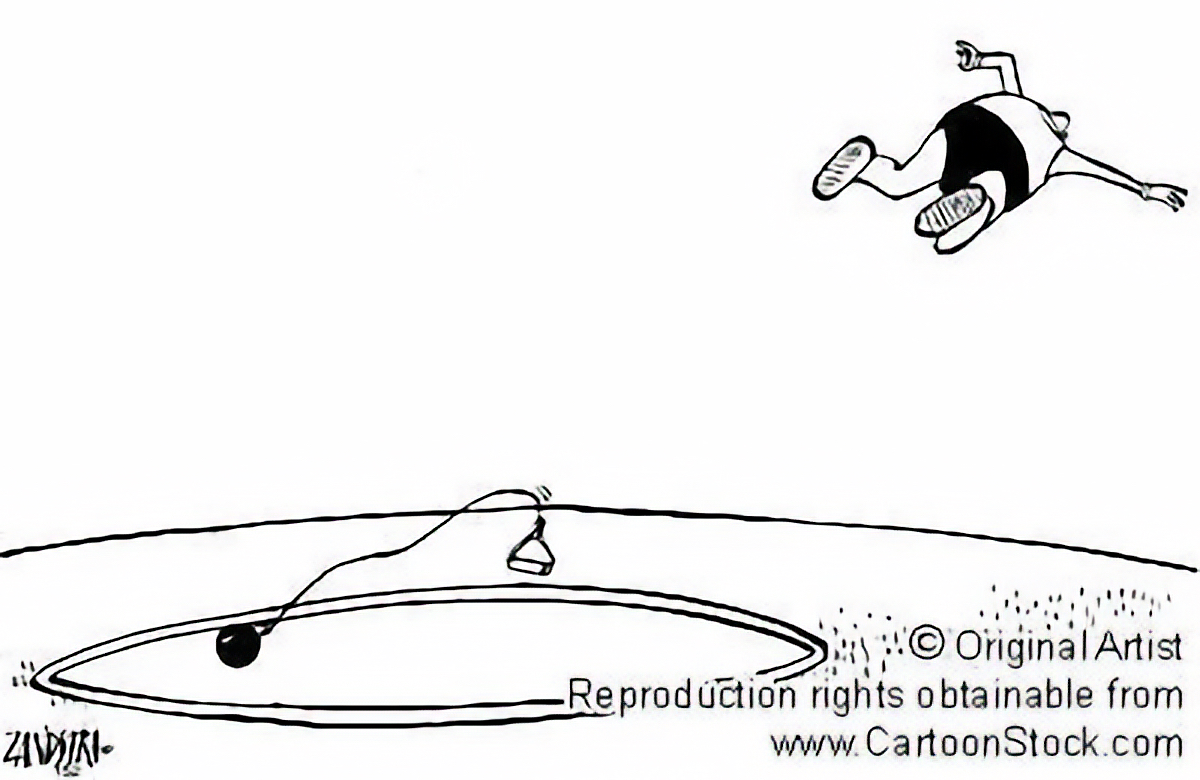
\includegraphics[width=\textwidth]{./dyn/exercises/jza0018l}%
		} 
\end{minipage}


\begin{oplossing}

De hamerslingeraar wordt weggeslingerd door de kogel stil blijft liggen. Het moet omgekeerd zijn.




ChatGPT

Waarom vliegt bij het hamerslingeren de kogel weg en niet de persoon?

Bij het hamerslingeren draait alles om de centripetale kracht die op de kogel (het hamerhoofd) wordt uitgeoefend wanneer het aan een draad wordt rondgedraaid voordat het wordt losgelaten. Laten we dit proces in meer detail bekijken:

1. **Centripetale kracht:** Wanneer de atleet het hamerhoofd rondzwaait, ervaart de kogel een centripetale kracht die naar het middelpunt van de cirkel is gericht (in dit geval het draaipunt van de draad). Deze kracht zorgt ervoor dat de kogel voortdurend naar het centrum van de cirkel wordt getrokken.

2. **Inertie van de persoon:** Tegelijkertijd ervaart de atleet, die de kogel rondzwaait, een tegenovergestelde reactie volgens de derde wet van Newton: "Actie is reactie". De atleet oefent een kracht uit op de kogel, maar de kogel oefent ook een gelijke maar tegengestelde kracht uit op de atleet.

3. **Massaverschil:** Het belangrijke verschil hier is het verschil in massa tussen de atleet en de kogel. De kogel heeft veel meer massa dan de atleet. Volgens de tweede wet van Newton (F = m * a), waarbij F de kracht is, m de massa en a de versnelling, zal de kogel minder versnellen dan de atleet, omdat de kracht gelijk is maar de massa veel groter is.

Samenvattend zorgt de centripetale kracht ervoor dat de kogel in een cirkelbaan blijft, terwijl de atleet, vanwege het massaverschil, veel meer versnelt dan de kogel. Daarom blijft de kogel rondzwaaien, terwijl de atleet niet wordt weggeslingerd.

\end{oplossing}

\end{exercise}
